\centerline{\bf \Huge Матбой}
\centerline{\bf \Huge Решения}

\problem{1}
На доске написаны числа $1^2, 2^2, \ldots, 100^2$. Найдите наименьшее натуральное число, на которое делятся ровно два из выписанных чисел.
%комол 8 класс утюм 1 задача

\textbf{Ответ: 34.}

\textbf{Решение:}
Для любого $n \leqslant 33$ на доске написаны числа $n^2,(2 n)^2$ и $(3 n)^2$, поэтому такое число не подходит. С другой стороны, если $k^2$ делится на $34=2 \cdot 17$, то $k$ делится на простые числа 2 и 17 и, следовательно, на их произведение 34 . Однако среди чисел от 1 до 100 на 34 делятся только два числа.

\problem{2}
В треугольнике $A B C$, в котором $\angle A=60^{\circ}$, проведена медиана $A M$. На продолжении стороны $A C$ за точку $C$ отмечена точка $N$ так, что $A M=M N$. Найдите $A B / C N$.
%комол 7 клас утюм 4 задача

\textbf{Ответ: $A B / C N=2$.}

\textbf{Решение:}
Удвоим медиану $A M$ : на продолжении луча $A M$ за точку $M$ отметим такую точку $D$, что $A M=M D$. Заметим, что $A B D C$ параллелограмм, в частности $A B=C D$ и $\angle D C N=\angle A=60^{\circ}$. С другой стороны, т.к. $A M=M D=M N$, то $\angle C N D=90^{\circ}$. Таким образом, в треугольнике $D C N$ один угол равен $60^{\circ}$, а другой $-90^{\circ}$. Поэтому $A B / C N=C D / C N=2$.

\problem{3}
Можно ли на гранях восьми одинаковых кубиков записать числа (не обязательно натуральные) так, чтобы из этих кубиков можно было составить вдвое больший куб с любой суммой от 1 до 10000000 на видимых гранях?

\textbf{Ответ: Можно}.

\textbf{Решение:}
У нас есть 24 пары противоположных граней. Пронумеруем их числами от 0 до 23 , и на гранях $k$-й пары запишем числа 0 и $2^k$. Так как $2^{24}>10000000$, то любая требуемая сумма однозначно представляется в виде суммы различных степеней двойки. Отметим на кубиках грани с нужными степенями, а для остальных степеней отметим противоположные грани. Тогда в каждом кубике будут отмечены ровно три грани с общей вершиной. Поместим его в большой куб отмеченными гранями наружу.

\problem{4}
Число $x^2+xy+y^2$ заканчивается на $\ldots0$ Докажите, что тогда оно заканчивается на $\ldots00.$

\textbf{Решение:}
Нам известно, что число $x^2+xy+y^2$ делится на 2 и на 5. Докажем, что тогда каждое из чисел $x$ и $y$ делится на 2 и на 5, откуда будет следовать требуемое.

Если число $x^2+xy+y^2$ четно, что очевидно, что числа $x$ и $y$ сами четны.

Далее, пусть $x^2+xy+y^2$ делится на 5. Если одно из чисел $x$ или $y$ делится на 5, то и другое тоже, очевидно, делится на 5. Пусть теперь ни $x$, ни $y$ на 5 не делятся. Тогда $x^2$, $y^2\equiv \pm 1 \ (mod \ 5)$. Если $x^2\equiv \pm 1 \ (mod \ 5)$ и $y^2\equiv \mp 1 \ (mod \ 5)$, то $xy$ делится на 5 --- противоречие. Значит, $x^2\equiv y^2\equiv \pm 1 \ (mod \ 5)$. Поэтому $xy\equiv \mp 2\ (mod \ 5)$. Но это возможно, только если $x\equiv \pm 2y \ (mod \ 5)$, а тогда $x^2\equiv -y^2 \ (mod \ 5)$ --- противоречие.

Итак, числа $x$ и $y$ делятся и на 2, и на 5, поэтому число $x^2+xy+y^2$ делится на 100, что и требовалось доказать.

\problem{5}
Положительные числа $x$, $y$, $z$ таковы, что $x+y+z=1/x+1/y+1/z$. Докажите, что $x+y+z\geq\sqrt{\dfrac{xy+1}{2}}+\sqrt{\dfrac{yz+1}{2}}+\sqrt{\dfrac{zx+1}{2}}$.

\textbf{Решение:}
По неравенству о средних для двух чисел имеем: $$\frac{x+1/y}{2}+y\geq \sqrt{\frac{x+1/y}{2}\cdot y}=2\sqrt{\frac{xy+1}{2}}.$$ Сложив это неравенство с двумя аналогичными, получаем: $$\frac{x+1/y}{2}+y+\frac{y+1/z}{2}+z+\frac{z+1/x}{2}+x\geq \sqrt{\dfrac{xy+1}{2}}+\sqrt{\dfrac{yz+1}{2}}+\sqrt{\dfrac{zx+1}{2}}.$$
Осталось заметить, что в левой части стоит выражение $$\frac 3 2 (x+y+z)+\frac 1 2 (\frac 1 x+\frac 1 y+\frac 1 z)=2(x+y+z),$$
что и завершает доказательство.

\problem{6}
Существует ли многочлен $f(x)$ четвертой степени с целыми коэффициентами такой, что для любого целого $k$ многочлен $f(x)+k$ не представляется в виде произведения двух квадратных трехчленов с целыми коэффициентами?

\textbf{Решение:}
Докажем, что можно выбрать многочлен $f(x)=x^4+x^2+x$. Предположим, что существует целое число $k$, такое, что $x^4+x^2+x+k=(x^2+ax+b)(x^2+cx+d)$, где $a$, $b$, $c$ и $d$ --- целые числа. Тогда $$a+c=0, \quad b+d+ac=1,\quad ad+bc=1.$$ Из первого равенства получаем, что $c=-a$, а из третьего --- что $a(d-b)=1$. Значит, или $a=1$ и $d=b+1$, или $a=-1$ и $d=b-1$. В первом случае второе равенство принимает вид $2b=1$, а во втором --- вид $2b=3$. Оба они невозможны при целом $b$.

\problem{7}
На летние сборы ЭлМШ пришли $n$ учеников, некоторые из которых знакомы друг с другом. Оказалось, что на сборах у каждого ученика не более $2k$ знакомых, но у каждых двух учеников, не знакомых друг с другом, не менее $k$ общих знакомых. Докажите, что $n \leq 6k$.

\textbf{Решение:}
Рассмотрим граф знакомств и подвесим его за любую вершину $A$. Пусть в первом слое будет $x$ вершин, тогда во втором --- $n-x-1$ вершин. Ясно, что $x\leq 2k$. Далее, рассмотрим вершину $A$ и произвольную вершину $B$ из второго слоя. По условию у них должно быть не менее $k$ общих соседей, однако находиться эти общие соседи могут только в первом слое. Значит, из вершины $B$ в первый слой ведет не менее $k$ ребер. 

Оценим общее количество ребер у вершин первого слоя. С одной стороны, их не более $2kx$, с другой стороны, не менее $x + (n-x-1)k$. Получаем неравенство $x+(n-x-1)k\leq 2kx$, откуда $n\leq x(3-1/k) + 1$. Вспоминая, что $x\leq 2k$, получаем $n\leq 2k(3-1/k)+1=6k-2+1\leq 6k$, что и требовалось доказать.

\problem{8}
В остроугольном треугольнике $A B C$ высоты $A D, B E$ и $C F$ пересекаются в точке $H.$ $P$ и $Q$ --- проекции точек $A$ и $H$ на $E F$ соответственно. Пусть $R$ - точка пересечения $D P$ и $Q H$. Докажите, что $HQ = HR$.

\textbf{Решение:}
По теореме о полном четырехстороннике для $A E H F$ четверка точек $(D, T, H, A)$ --- гармоническая. Теперь спроецируем эту четверку на прямую QR через точку $P$ и получим, что
$$
-1 = (D, T, H, A) = (R, Q, H, \infty_{QR}) = \dfrac{\overrightarrow{RH}}{\overrightarrow{QH}}
$$

Точка $A$ отобразилась в бесконечно удалённую точку по направлению к $QR$, так как $PA \| QR.$ Равенство $\dfrac{\overrightarrow{RH}}{\overrightarrow{QH}}=-1$ и даёт требуемое.

\begin{center}
    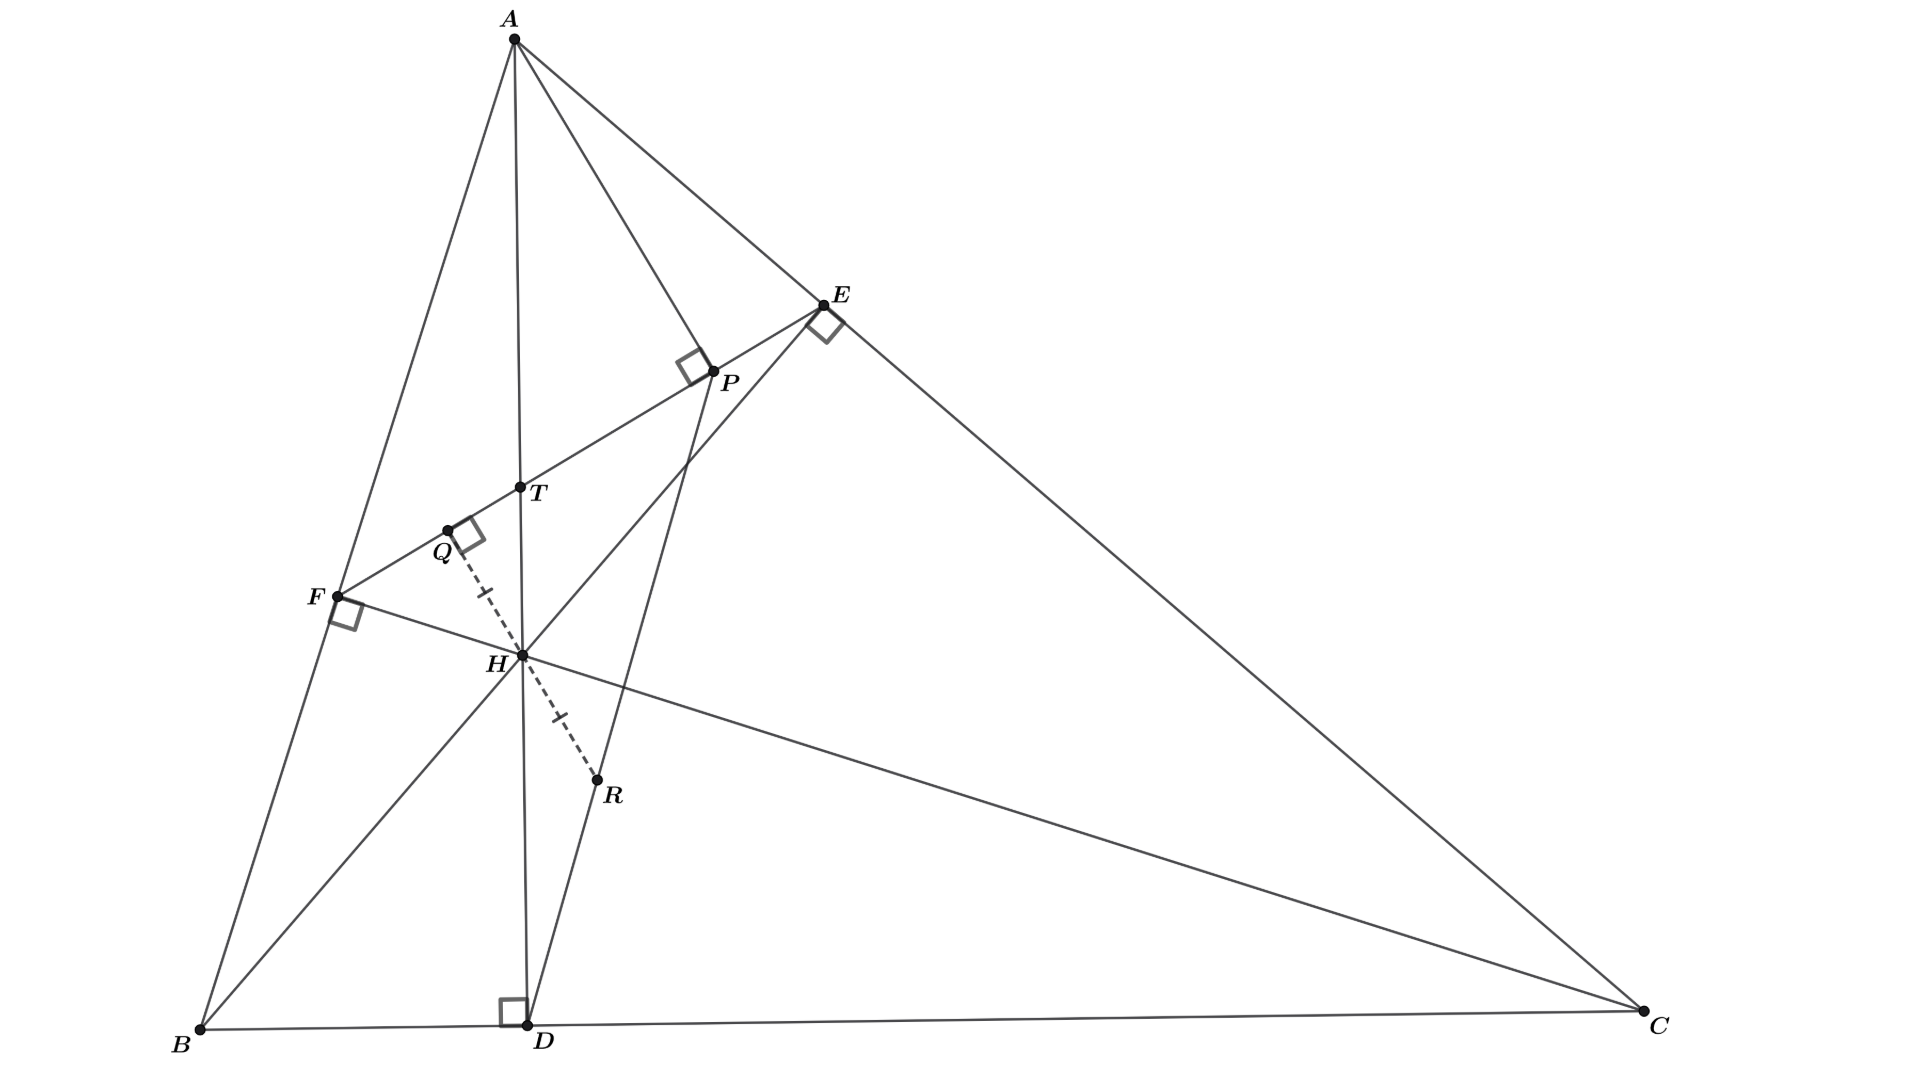
\includegraphics[width=1\textwidth]{Сборы/Сборы Элиста 2025/РВ/10/battle_sol_8.png}
\end{center}